\documentclass[letterpaper,11pt]{article}

% Soporte para los acentos.
\usepackage[utf8]{inputenc}
\usepackage[T1]{fontenc}
% Idioma español.
\usepackage[spanish,mexico, es-tabla]{babel}
% Soporte de símbolos adicionales (matemáticas)
\usepackage{multirow}
\usepackage{amsmath}
\usepackage{amssymb}
\usepackage{amsthm}
\usepackage{amsfonts}
\usepackage{mathtools}
\usepackage{latexsym}
\usepackage{enumerate}
\usepackage{ragged2e}
\usepackage{listings}
\usepackage{xcolor}
\usepackage{graphicx}
\usepackage{hyperref}
\usepackage[linguistics]{forest}
\usepackage{algorithm}
\usepackage{algpseudocode}

% Modificamos los márgenes del documento.                                       %
\usepackage[lmargin=2cm,rmargin=2cm,top=2cm,bottom=2cm]{geometry}

\definecolor{codegreen}{rgb}{0,0.6,0}
\definecolor{codegray}{rgb}{0.5,0.5,0.5}
\definecolor{codepurple}{rgb}{0.58,0,0.82}
\definecolor{backcolour}{rgb}{0.95,0.95,0.92}

\lstdefinestyle{mystyle}{
    backgroundcolor=\color{backcolour},   
    commentstyle=\color{codegreen},
    keywordstyle=\color{magenta},
    numberstyle=\tiny\color{codegray},
    stringstyle=\color{codepurple},
    basicstyle=\ttfamily\footnotesize,
    breakatwhitespace=false,         
    breaklines=true,                 
    captionpos=b,                    
    keepspaces=true,                 
    numbers=left,                    
    numbersep=5pt,                  
    showspaces=false,                
    showstringspaces=false,
    showtabs=false,                  
    tabsize=2
}

\lstset{style=mystyle}

\title{Facultad de Ciencias, UNAM \\ Análisis de Algoritmos \\ Tarea 1}
\author{Rubí Rojas Tania Michelle}
\date{09 de octubre de 2020}

\begin{document}
\maketitle

\begin{enumerate}
    % Ejercicio 1.
    \item ¿Cuántas comparaciones son necesarias y suficientes para ordenar 
    cualquier lista de cinco elementos? Justifique su respuesta.

    \textsc{Solución:} Un árbol de decisión es un árbol binario completo que 
    representa las comparaciones realizadas en todas las ejecuciones posibles 
    sobre entradas de tamaño $n$. Cada nodo interno se representa de la forma 
    $i:j$ con $1 \leq i < j \leq n$ y cada hoja con una permutación 
    $\langle \pi(1), \pi(2), ..., \pi(n) \rangle$ sobre $\{1, 2, ..., n\}$.

    La ejecución del algoritmo de ordenamiento sobre una entrada dada 
    corresponde a un camino en el árbol desde la raíz hasta la hoja. Dicho 
    camino denota las comparaciones realizadas y su órden de realización para 
    la entrada. Es decir, un nodo $i:j$ en el camino denota la comparación 
    $a_i \leq a_j$. Si el camino continúa sobre el hijo izquierdo, la
    comparación es cierta y si continúa sobre el hijo derecho entonces la 
    comparación es falsa. Si la entrada alcanza la hoja $\langle \pi(1), 
    \pi(2), ..., \pi(n) \rangle$, entonces la permutación de entrada ordenada 
    es $\langle a_{v\pi(1)}, a_{\pi(2)}, ..., a_\pi(n) \rangle$.

    Un ejemplo de árbol de decisión sería el siguiente:
    \begin{figure}[h]
        \centering
        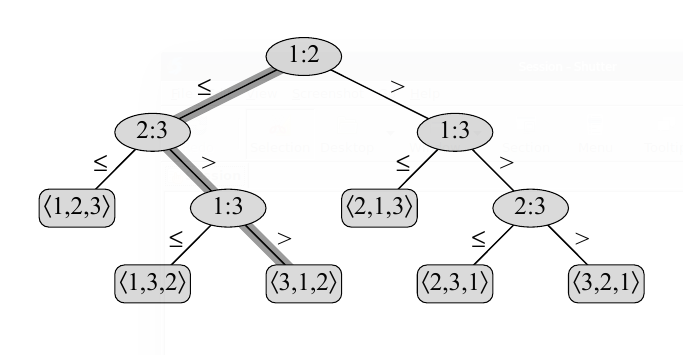
\includegraphics[width=0.5\linewidth]{imagenes/decision-tree.png}
        \caption{Árbol de decisión correspondiente a tres elementos (Cormen, 
        192 pag.)}
        \label{fig:decision-tree}
    \end{figure}

    La entrada corresponde a $\langle a_1, a_2, a_3 \rangle = \langle 6, 8, 5, 
    \rangle$. Lo primero que hace es la comparación $a_1 \leq a_2$, que es 
    cierta. Luego se compara $a_2 \leq a_3$, que es falsa. Finalmente compara 
    $a_1 \leq a_3$, que también es falsa. La entrada ordenada es $\langle 5, 6, 
    8 \rangle$. Notemos que hay $3! = 6$ posibles permutaciones en la entrada 
    de elementos, por lo que el árbol de decisión tiene $6$ hojas.

    Ahora bien, de manera más general, digamos que para $n$ elementos tenemos 
    un árbol de decisión $T$ de altura $h$ y con $l$ hojas alcanzables. Como el 
    árbol ordena las $n!$ distintas permutaciones, entonces el árbol contiene 
    una hoja por cada una de las $n!$ permutaciones, por lo que $n! \leq l$. 
    Como un árbol binario de altura $h$ tiene a lo más $2^h$ hojas, entonces 
    $n! \leq l \leq 2^h$, de donde 
    \begin{align*}
        2^h &\geq n!
        && \text{por transitividad} \\
        \log_2 (2^h) &\geq \log_2 (n!)
        && \text{tomando los logaritmos} \\
        h &\geq \log_2 (n!)
        && \text{propiedad de logaritmo} \\
        &= \log_2 (n \cdot (n-1) \cdot (n-2) \cdot (n-3) \cdots \cdot 3 \cdot 
        2 \cdot 1)
        && \text{definición de factorial} \\ 
        &= \log_2 (n) + \log_2 (n-1) + \log_2 (n-2) + \log_2 (n-3) +
        && \text{propiedad de logaritmo} \\ 
        & \; \; \; \; \;  \cdots + \log_2 (3) + \log_2 (2) + \log_2 (1) \\
        &= \int_1^n \! \log_2 (x) \, \mathrm{d}x.
        && \text{es el área bajo la curva} \\ 
        &= x \log_2 (x) - x \Big|_1^n
    \end{align*}

    Es decir, en el peor de los casos tenemos que hacer $x \log_2 (x) - x 
    \Big|_1^n$ comparaciones. Por lo tanto, para ordenar una lista de $5$ 
    elementos son \textit{necesarias} $7$ comparaciones. 

    % Ejercicio 2.
    \item Dados dos arreglos ordenados $A$ y $B$ de longitud $n$ y $m$, 
    respectivamente. Diseña un algoritmo de tiempo $O(n + m)$ que obtenga un 
    arreglo $C$ que contenga los elementos en común entre $A$ y $B$, $C$ no 
    debe tener elementos repetidos.

    \textsc{Solución:} El algoritmo propuesto para resolver este problema es 
    el siguiente
    \begin{center}
    \begin{minipage}[c]{0.7\textwidth}
    \begin{algorithm}[H]
        \caption{Obtener los elementos en común entre los arreglos $A$ y $B$} 
        \begin{algorithmic}[1]
            \State $i \gets 0$
            \State $j \gets 0$
            \State $C = []$
            \While {$(i < n$ \textbf{and} $j < m)$}
                \If {$A[i] == B[j]$}
                    \If {$C.length > 0$ \textbf{and} $C[C.length - 1] == A[i]$}
                        \State $i \gets i + 1$
                        \State $j \gets j + 1$
                    \Else
                        \State $C.append[A[i]]$
                        \State $i \gets i + 1$
                        \State $j \gets j + 1$
                    \EndIf
                \Else \If {A[i] < A[j]}
                    \State $i \gets i + 1$
                \Else
                    \State $j \gets j + 1$
                \EndIf
                \EndIf
            \EndWhile
        \end{algorithmic} 
    \end{algorithm}
    \end{minipage}
    \end{center}
   
    Primero, explicaremos porqué el algoritmo funciona. En las líneas $(1 - 2)$ 
    estamos definiéndo dos variables $i, j$; las cuales nos ayudarán a recorrer
    los arreglos $A$ y $B$, respectivamente. En la línea $3$ simplemente creamos 
    a nuestro arreglo $C$. A partir de la línea $4$ empieza lo interesante: como
    sabemos que los arreglos $A$ y $B$ están ordenados, eso significa que 
    tenemos que checar tres casos en específico:
    \begin{enumerate}
        \item (líneas $(5 - 13)$). Si el $i-$ésimo elemento de $A$ es igual al 
        $j-$ésimo elemento de $B$ eso significa que tienen un elemento en común 
        y, en teoría, se debe agregar al arreglo $C$. Pero antes de agregarlo,
        comprobamos que no esté repetido en $C$: para verificar esto simplemente
        hay que ver si el elemento $A[i]$ (o $B[j]$) es igual al último elemento 
        que fue agregado a $C$ (como $A$ y $B$ están ordenados, si es que tienen 
        elementos repetidos, entonces éstos están juntos). Si el elemento ya se 
        encuentra en $C$ entonces simplemente incrementamos nuestros contadores 
        en \textit{uno}; en caso contrario, agregamos al elemento a $C$ e 
        incrementamos los contadores en \textit{uno}.

        \item (líneas $(15 - 16)$). Si el $i-$ésmo elemento de $A$ es menor que 
        el $j-$ésimo elemento de $B$, eso quiere decir que debemos movernos un 
        índice a la derecha en el arreglo $A$; ya que como están ordenados ambos 
        arreglos, eso quiere decir que, si tienen elementos en común, entonces 
        éste (o éstos) son mayores que el $i-$ésimo elemento de $A$.

        \item (línea $18$). Aquí cae el caso en que $B[j] < A[i]$, y 
        análogamente al caso anterior, tenemos que movernos un índice a la 
        derecha en el arreglo $B$; ya que como están ordenados ambos arreglos, 
        eso quiere decir que, si tiene elementos en común, entonces éste (o 
        éstos) son mayores que el $j-$ésimo elemento de $B$. 
    \end{enumerate} 

    Todo esto se realizará hasta que la condición de nuestro \textit{while} 
    (línea $14$) se cumpla: como $n$ puede ser diferente de $m$, lo que hay 
    que tener en cuenta es que si terminamos de recorrer un arreglo, entonces 
    debemos terminar el proceso. Esto se debe al hecho de que los arreglos
    están ordenados. Si terminamos de recorrer un arreglo, entonces ya no 
    habrá más elementos en común, es decir, podríamos recorrer un arreglo sin 
    terminar de recorrer al otro; pero en el peor caso, debemos recorrer 
    completamente ambos arreglos, por este motivo la complejidad de nuestro 
    algoritmo es $O(n + m)$. 

    % Ejercicio 3.
    \item Consider the following sorting algorithm:
    \begin{figure}[ht]
        \centering
        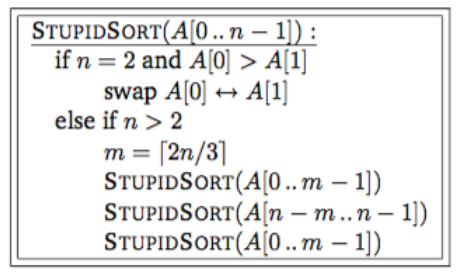
\includegraphics[width=0.4\textwidth]{./imagenes/stupidSort.png}
    \end{figure}

    \begin{enumerate}
        % Ejercicio 3.1
        \item Prove that \textsc{stupidsort} actually sorts its input.

        % Ejercicio 3.2
        \item Would the algorithm still sort correctly if we replaced 
        $m = \lceil \frac{2n}{3}\rceil$. Justify your answer.

        % Ejercicio 3.3
        \item Show that the number of swaps executed by \textsc{stupidsort} is
        at most $\big(\begin{smallmatrix} n \\ 2 \end{smallmatrix}\big)$.
    \end{enumerate}

    % Ejercicio 4.
    \item Supongamos que tenemos que ordenar una lista $L$ de $n$ enteros cuyos
    valores están entre $1$ y $m$. Pruebe que si $m$ es $O(n)$ entonces los 
    elementos de $L$ pueden ser ordenados en tiempo lineal. ¿Qué pasa si $m$ es 
    de $O(n^2)$? ¿Se puede realizar en tiempo lineal? ¿Por qué?

    % Ejercicio 5.
    \item Describe an algorithm that, given $n$ integers in the range $0$ to 
    $k$, preprocesses its input and then answers any query about how many of 
    the $n$ integers fall into a range $[a ... b]$ in $O(1)$ time. Your 
    algorithm should use $\Theta(n + k)$ preprocessing time.

    \textsc{Solución:}

    % Ejercicio 6.
    \item Sea $A$ un arreglo de $n$ elementos, tal que cada elemento se 
    encuentra a lo más a $k$ posiciones de su posición ordenada. Diseñe un 
    algoritmo que ordene $A$ en $O(n \log k)$.

    % Ejercicio 7.
    \item An abs-sorted array is an array of numbers in which $|A[i] \leq A[j|$
    whenever $i < j$. For example, the array $A = [-49, 75, 103, -147, 164, -197,
    -238, 314, 348, -422]$, though not sorted in the standard sence, is 
    abs-sorted. Design and algorithm that takes an abs-sorted array $A$ and a 
    number $k$, and returns a pair of indices of elements in $A$ that sum up to 
    $k$. For example, if $k = 167$ your algorithm should output $(3, 7)$. Output 
    $(-1, -1)$ if the is no such pair.

    % Ejercicio 8.
    \item \textbf{The Hogwarts Sorting Hat}

    Every year, upon their arrival at Hogwarts School of Witchcraft and Wizardry, 
    new students are sorted into one of four houses (Gryffindor, Hufflepuff, 
    Ravenclaw, or Slytherin) by the Hogwarts Sorting Hat. The student puts the 
    Hat on their head, and the Hat tells the student which house they will join. 
    This year, a failed experiment by Fred and George Weasley filled almost all 
    of Hogwarts with sticky brown goo, mere moments before the annual Sorting. 
    As a result, the Sorting had to take place in the basement hallways, where 
    there was so little room to move that the students had to stand in a long 
    line. After everyone learned what house they were in, the students tried to 
    group together by house, but there was too little room in the hallway for 
    more than one student to move at a time. Fortunately, the Sorting Hat took 
    Algorithms many years ago, so it knew how to group the students as quickly 
    as possible. What method did the Sorting Hat use? More formally, you are 
    given an array of n items, where each item has one of four possible values, 
    possibly with a pointer to some additional data. Design and analyze an 
    algorithm that rearranges the items into four clusters in $O(n)$ time 
    using only $O(1)$ extra space.

    \newpage
    % Ejercicio 8.
    \item Pruebe que el segundo elemento más chico de una lista de $n$ elementos 
    distintos puede encontrarse con $n + \lceil \log n \rceil - 2$ comparaciones.

    \begin{proof}
        Sea $T$ el árbol binario, en particular un \textit{min-Heap}, que 
        contiene a los $n$ elementos de nuestra lista en sus hojas. Por lo 
        discutido en clase, sabemos que para encontrar al elemento más pequeño 
        necesitamos realizar $n-1$ comparaciones, ya que al ir comparando los 
        elementos desde las hojas, vamos formando nuestros nodos internos (éstos 
        serán los elementos más pequeños de las comparaciones que se vayan 
        haciendo), los cuales siempre son $n-1$.

        Ahora bien, para encontrar al segundo elemento más pequeño debemos
        tener en cuenta una observación importante: como siempre vamos 
        \textit{subiendo} a los elementos más pequeños, eso quiere decir que el 
        segundo elemento más pequeño ya fue comparado con la raíz del árbol $T$,
        así que sólo queda ubicar a todos los elementos que \textit{perdieron}
        contra la raíz de $T$ y compararlos entre sí. Al ubicar estos elementos, 
        obtendremos que hay uno de ellos (a lo más) en cada nivel del árbol, y 
        como la altura del árbol es $\log_2 n$ entonces hacer esta última 
        pasada al árbol nos tomará $\lceil \log_2 n \rceil - 1$ comparaciones.
        Por lo tanto, encontrar al segundo elemento más pequeño de una lista de 
        $n$ elementos distintos nos toma 
        \begin{equation*}
            (n - 1) + (\lceil \log_2 n \rceil - 1) = n + \lceil \log_2 \rceil - 2
        \end{equation*}

        comparaciones.

        \begin{figure}[ht]
        \centering
        \forestset{default preamble={for tree={circle,draw}}}
        \begin{forest}
        [-1, red
          [-1,
            [-1
              [24, blue]
              [-1]
            ]
            [2, blue
              [2]
              [7]
            ]
          ]
          [0, blue
            [9]
            [0]
          ]
        ]
        \end{forest}
            
        \caption{Ejemplo de la explicación con la lista $[24, -1, 2, 7, 9, 0]$.
                 Los elementos en azul son aquellos que \textit{perdieron} contra 
                 el elemento más pequeño.}
        \end{figure}
    \end{proof}

\end{enumerate}
\end{document}
